\vspace{12pt}
\section{Electrical Properties of Doped Barium Zirconate Thin Film Samples}
Similarly to the methods used to test the conductivity of bulk samples, the films were studied using impedance spectroscopy to gather conductivity data over a range of temperatures by applying contacts and electrical leads. Impedance arcs are then fit using a complex non-linear least squares method to equivalent circuit models to obtain resistance values of the film. In the case of these films, only one arc is obtained, and the resistance extracted is attributed to the total conduction through the film. Separation of grain interior and grain boundary contributions is not possible. In order to calculate conductivity from the resistance data, a geometrical constant is needed. For the case of these thin films, this is based on the geometry similar to that of the ``in-plane’’ geometry of Figure \ref{fig:bulk:geometry}b for bulk samples. Unlike for the bulk case, this geometry allows for an accurate assessment of the conductivity since the films are much thinner than the distance between the contacts. Therefore, the geometrical constant can be calculated by
\begin{equation}
    \frac{A}{l} = \frac{\textrm{film thickness} \times \textrm{length of contact stripe}}{\textrm{distance between contacts}}.
\end{equation}
Our contacts were deposited with silver paint 2 mm apart and 8 mm long. All films tested in this chapter were deposited with 9000 pulses at a laser energy density of 2.8 J/cm$^2$ which at a deposition rate of 0.8 \AA/pulse gives a thickness of 720 nm. combining these dimensions gives a geometrical factor $A/l=0.0003$ cm. 

Figure \ref{films:fig:ny:praxBZG850} shows typical impedance measurements obtained for thin films in ambient air. In this case the film was deposited at 850\textdegree C with a laser fluence of 2.8 J/cm$^2$ and an oxygen background pressure of 50 mTorr.  The effect of temperature on the overall resistance of the sample is clearly noted with the diameter of the semi-circular arcs decreasing with increasing temperature. The single arc observed for each temperature is consistent with a single relaxation frequency and ionic transport mechanism. All arcs are consequently well described by a simple parallel RC model.  After RC model fitting, and extraction of accurate values of resistance, the conductivity for each temperature was obtained using the geometrical parameters of our setup. The resulting temperature dependence of the conductivity of this typical film is shown in Figure \ref{films:fig:arr:praxBZGair}. A simple fit of the Arrhenius plot obtained yields an activation energy of 0.40 eV for the conduction process in this film.
\begin{figure}
\centering
\begin{subfigure}{.9\linewidth}
    \centering
    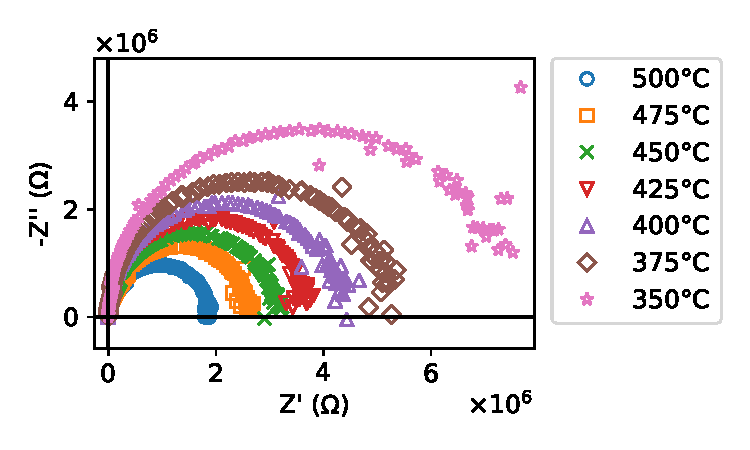
\includegraphics{Figures/180522-film-PraxBZG-850-air-nyquist.pdf}
    \caption{}
    \label{films:fig:ny:praxBZG850}
\end{subfigure}
\\
\vspace{.4in}
\centering
\begin{subfigure}{.9\linewidth}
    \centering
    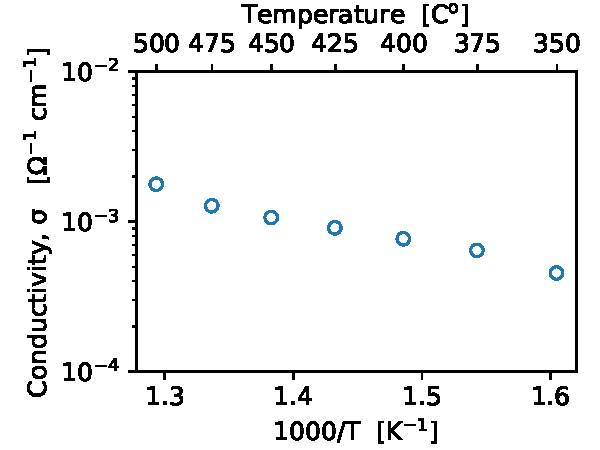
\includegraphics{Figures/180522-film-PraxBZG-850-air.pdf}
    \caption{}
    \label{films:fig:arr:praxBZGair}
\end{subfigure}
\caption{(A) Nyquist plot for thin film sample deposited at 850\textdegree C with a laser energy density of 2.8 J/cm$^2$ using a Gd:BaZrO\textsubscript{3} target produced by combustion spray pyrolysis. Temperature dependent resistance is clear from the decrease in Z' axis intercept with increasing temperature. (B) Arrhenius plot of the resistances extracted from Fig A using the geometrical factor to calculate conductivity. Fitting for the data accounting for temperature dependence as in equation \ref{arrhenius} gives an activation energy of 0.40 eV, that agrees well with similar proton conducting solids in the literature.}
\end{figure}


% \begin{figure}
%     \centering
%     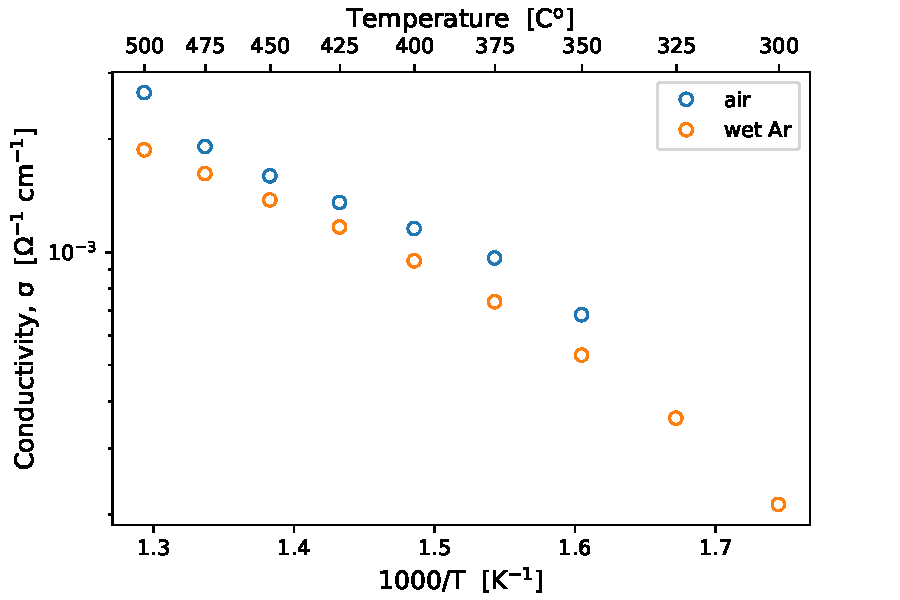
\includegraphics[width=\textwidth]{Figures/PraxBZG-film-850-comparison-gas-env.pdf}
%     \caption{This will contain the collection of gas environment Arrhenius plots for film deposited at 850\textdegree C.}
%     \label{films:fig:arr:praxBZGgas}
% \end{figure}

Testing the effect of different gaseous environment was another important step in validating the conduction mechanism as well as demonstrating some consistency of behavior between the bulk samples and the thin films which derived from them. Figure \ref{films:fig:arr:180201:gas} compares the conductivity for a film made with a deposition temperature of 950\textdegree C in different chemical gaseous environments. These measurements were made under conditions of ambient air, dry argon, humidified forming gas (5\% H$_2$ in N$_2$ balance), and then retested in several times in this environment to check consistency. 

\begin{figure}
    \centering
    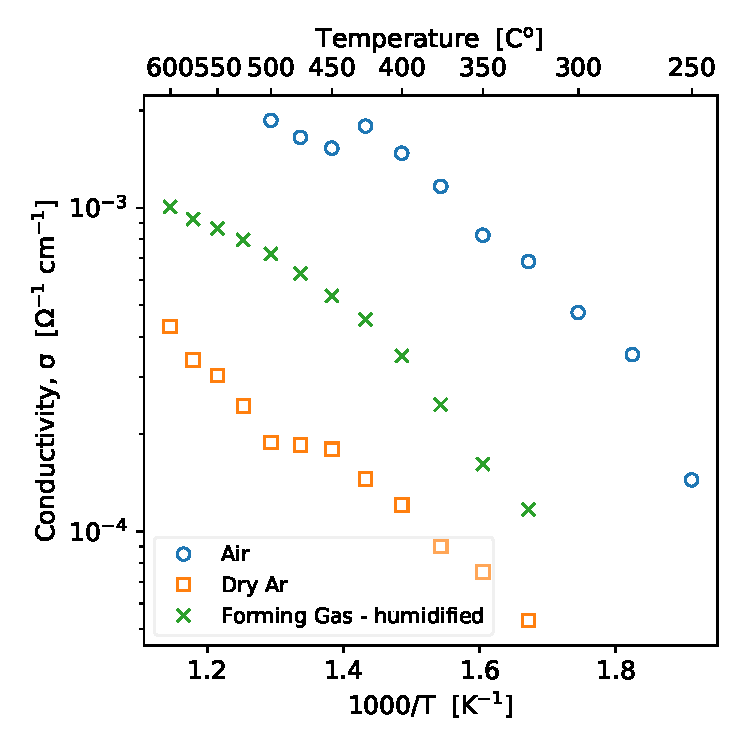
\includegraphics{Figures/180821-film-180201-gas-change.pdf}
    \caption{Comparison of gaseous environment on conductivity of film deposited at 950\textdegree C on MgO substrate with pellet synthesized by combustion spray pyrolysis.}
    \label{films:fig:arr:180201:gas}
\end{figure}

As with the bulk samples, these gaseous environments cause different responses in the conductivity of the films. In the dry argon environment oxygen vacancies are expected to form and the film will thus lack proton incorporation. Conductivity is lowered in this case, and that which is present may be the result of oxide ion conduction, particularly at higher temperatures. In the humid, reducing environment of humidified forming gas, proton incorporation is promoted and conductivity increases. A further increase in conductivity is noted when the experiment is repeated in air. Several possible mechanisms could be at work in this case which warrant further investigation. The oxidizing environment presented by introducing air could be filling oxygen vacancies by producing electron holes as shown in equation \ref{eq:bulk:holeConduction}. This hole conduction is expected at higher temperatures. The second possibility is that the reducing environment of the humidified forming gas is actually promoting oxygen vacancies by removing some oxides from the film, so that while there is proton conduction, the concentration of protons is not optimal due to unfilled vacancies. This would mean that the use of humid air could provide a balance of oxygen vacancy filling and proton availability that maximizes proton incorporation and thus conduction. 

\vspace{12pt}
\section{Effect of Dopant on Electrical Properties}
The bulk pellets made by solid state reaction as well as the pellet produced by combustion spray pyrolysis and characterized in Chapter \ref{ch:bulk} were used to deposit these films. The different dopants present in each are expected to have an effect on the conduction within each film. The structural differences in the films across different dopants will also have a (possibly larger) effect than the dopants themselves. Figure \ref{fig:films:eis:dopantComparison} shows the results of impedance spectroscopy for this films across different dopants, all in a humidified forming gas environment. As expected, the undoped film shows very little conductivity and very little change in response to temperature. It should be noted that the measured resistance at low frequency for this film is beyond the limits of the particular impedance analyzer in our apparatus. These conductivity values are the result of fitting equivalent circuits to the high frequency portion of the spectrum, but this film has essentially no conduction from the standpoint of measurement limits. Similarly, the ytterbium doped sample shows effectively no conduction. Although the bulk pellet with ytterbium doping showed lower conductivity than that of either yttrium or gadolinium it is unknown whether this conductivity is simply too low in the case of these films to detect or whether the difference in lattice parameter seen in the XRD results of Table \ref{tab:film:dopant:latticeParam} indicate a dopant incorporation that is not ideal. 
\begin{figure}
    \centering
    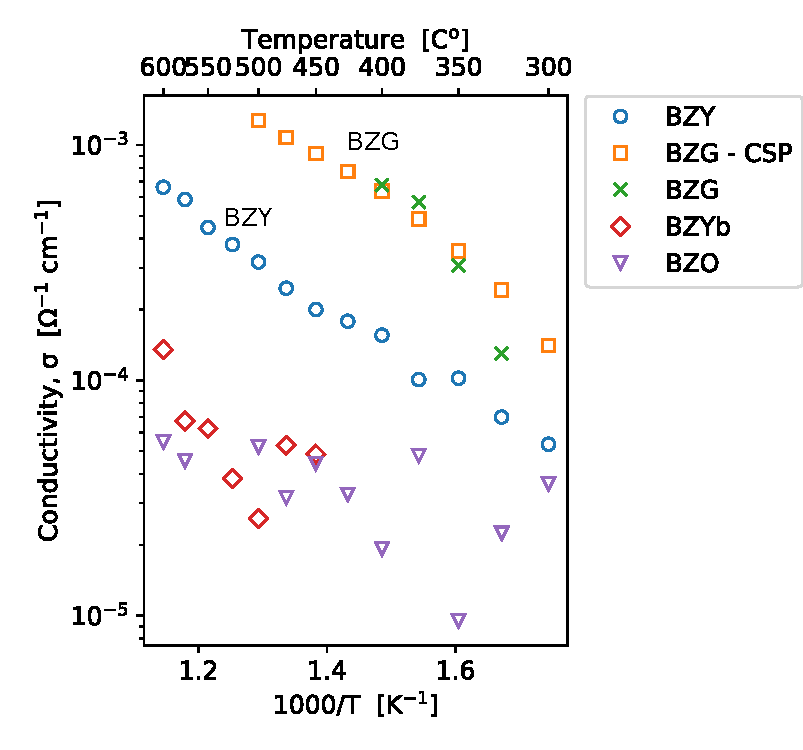
\includegraphics{Figures/190619-eis-film-dopant-comparison-edit-3.pdf}
    \caption{Comparison of films made with dopants from pellets characterized in Chapter \ref{ch:bulk}. ``BZO’’ here refers to undoped sample of pure BaZrO\textsubscript{3}. The target produced by combustion spray pyrolysis is noted as ``BZG - CSP.'' All films were tested in humidified forming gas environment.}
    \label{fig:films:eis:dopantComparison}
\end{figure}

Of significant note is the comparison of conductivities between yttrium and gadolinium. While the data for the gadolinium doped film made from in house produced target is limited, it is similar to the sample prepared from the combustion spray pyrolysis target which was tested over the full temperature range. With the exception of the ytterbium sample, the similarities in lattice parameters of these samples suggests that the films are strained by the substrate. But these similarities are enough that it is reasonably likely the differences in conductivity are due to the effect of the choice of dopant in the film. The interaction of the proton with that dopant is a plausible mechanism for this difference. For these preparations, the gadolinium doped sample is higher in conductivity, notably higher than the yttrium doped sample. These results are consistent with the proton-dopant interaction model discussed in Chapter \ref{ch:background}, that shows for dopants that cause a smaller distance between the proton and an adjacent dopant ion, the binding energy is higher and thus the proton spends more time in these trap sites. 

\vspace{12pt}
\section{Effect of Thin Film Microstructure on Conductivity}
\label{sec:conduction:epitaxy}
The microstructure of a thin film is bound to have substantial effect on its overall ionic conductivity. Changes in crystallite size, and number of grain boundaries alter the relative contributions of conduction by the grain interiors and grain boundaries. A parameter that was noted as having significant impact on grain boundaries and crystallite size in the substrate temperature. As observed in Figures \ref{fig:film:xrd:2theta} through \ref{fig:films:xrd:2thetaOmega:offset:750}, changes in substrate temperature in the 750-950\textdegree C range cause the Gd-doped thin films grown on MgO to change from an essentially random polycrystalline pattern at 750\textdegree C to an epitaxially-oriented single crystal (or highly textured structure) at 950\textdegree C. Given this strong indication of epitaxial growth from the X-ray diffraction studies discussed in \ref{sec:film:xrd:epitaxy}, it follows to test the effects of this change from random crystalline orientation to the essentially epitaxially grown film. These films were produced from the target made by combustion spray pyrolysis. The results of impedance spectroscopy carried out with air as the gaseous environment, along with the corresponding $\theta-2\theta$ XRD patterns for the samples are shown in Figure \ref{fig:film:eis:eis_xrd_comparison}.
\begin{figure}
    \begin{subfigure}{.9\linewidth}
        \centering
        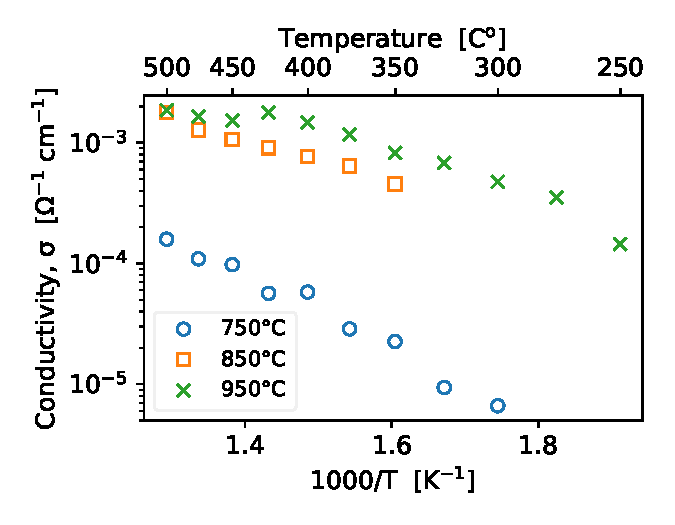
\includegraphics{Figures/181008-PraxBZG-film-comparison-air.pdf}
        \caption{}
        \label{fig:film:eis:eis_xrd_comparison}
    \end{subfigure}
    \\
    \vspace{.125in}
    \begin{subfigure}{.9\linewidth}
        \centering
        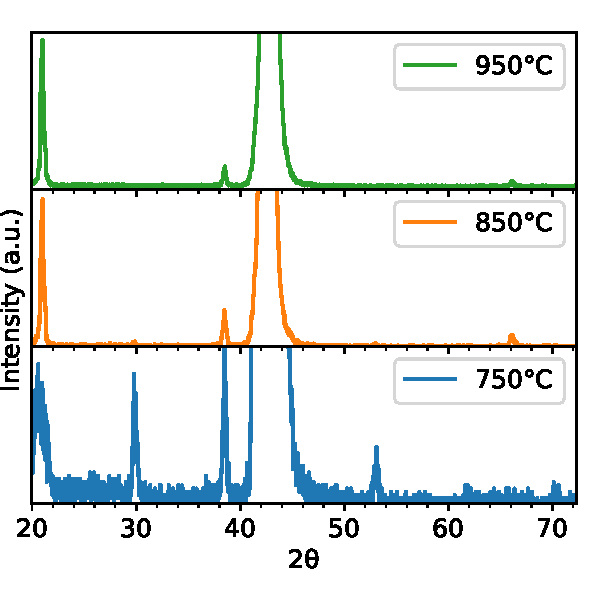
\includegraphics{Figures/181008-PraxBZG-film-comparison-xrd-zoom.pdf}
        \caption{}
        \label{fig:film:xrd:eis_xrd_comparison}
    \end{subfigure}
    \caption{Comparison of results of impedance testing with XRD of films showing significant crystallographic texture.}
\end{figure}
The EIS data reveals that this change is accompanied by an increase in thin film conductivity. The difference in conductivity from the film grown at 750\textdegree C to the one deposited at 850\textdegree C is the most dramatic, corresponding to a factor of 10 in conductivity increase. Since the 850\textdegree C sample already exhibits significant texturing, with major intensity reductions in the reflections from the (110) and (211) planes, this is likely due to a diminished resistance from blocking grain boundaries. The epitaxially-oriented thin film grown at 950\textdegree C shows further increase in conductivity, although a narrowing of the difference in conductivities between the 850\textdegree C and 950\textdegree C samples seems to exist for measuring temperatures approaching 500\textdegree C. These observations support the notion that crystallographic texture would affect the ionic conductivity of doped barium zirconate thin films, which was in part a motivation for this dissertation research.

The increase in conductivity that occurs with a decrease in random orientation of the crystalline structure can be understood given the discussion on the difference in conductivity between grain interiors and grain boundaries. In the limiting case, if the epitaxial sample could be shown to represent a grain-boundary-free material, then the conductivity of such an epitaxial film would be the conductivity through the bulk of the grain interiors, with complete elimination of the blocking grain boundary contribution.

\vspace{12pt}
\section{Conclusion}
Thin films with different dopants were grown and characterized under different deposition conditions, some of which were found to result in highly textured or epitaxial film growth. Namely, the substrate temperature during deposition was found to greatly change the crystallinity of the resulting films. 

The crystallographic structure of these films was measured for a variety of dopants (Yb, Y, Gd) and the growth rate was obtained by interference methods and scanning electron microscopy. This resulted in the determination of the index of refraction, which has not been directly reported in this way in the literature.

The conductivity of these films was investigated along several dimensions. The effect of gaseous environment was found to have dramatic effects on the conductivity, suggesting incorporation of ions to be the mechanism of conduction. The conductivity of films prepared with different dopants was also measured, and gadolinium doped films showed the highest conductivity of the films prepared. These conductivities are comparable with those reported for yttrium doped barium zirconate by Kim \cite{Kim2011} though lower than those reported Pergolesi \cite{Pergolesi2010}. Gadolinium and ytterbium doped barium zirconate thin films have been synthesized for the first time and the results of their conductivity values as thin films compared to yttrium doped films are consistent with the available theoretical models of proton trapping through association with the dopant ion \cite{Stokes2010}. 

The conductivity was measured to increase with increasing crystallographic texture as shown by X-ray diffraction analysis. Epitaxial growth of thin films were achieved on lattice matched MgO substrates under conditions of increased substrate temperature during deposition. This epitaxial growth led to an order of magnitude increase in the conductivity. Future work should involve analysis of films made through a wider range of deposition temperatures, as well as obtaining more information of the microstructure of these films by X-ray diffraction techniques such as reciprocal space mapping to determine mosaicity of grains. Expanding the range of impedance measurement by adding modules that support ultra low current measurement will also improve certainty of measurements as well as support measurement of ultra thin films that are more likely to be grown as true single crystalline structures.